\documentclass[a4paper]{article}
\usepackage{amsfonts}
\usepackage{amsmath}
\usepackage{amssymb}
\usepackage{graphicx}     

\begin{document}
  
\noindent \large Auteur: Sabawoon Enayat \\
\noindent \large Studierichting: Informatica\\
\noindent \large Oefeningenreeks 5D nr. 4.11 \\

\newcommand{\dint}{\displaystyle\int}

\medskip

\normalsize

Opgave: $y_1 = x^3 + 1$ en $y_2 = x^2 + x + 1$\\

$\Rightarrow y_1 = y_2 \Rightarrow y_2 - y_1 = 0 \Rightarrow \left(x^2 + 2x + 1\right) - \left(x^3 + 1\right) = 0$\\

$\Rightarrow -x^3 + x^2 + 2x = 0 \Rightarrow x\left(-x^2 + x + 2\right) = 0$\\

$D = 1 - 4 \cdot (-1) \cdot 2 = 9 \Rightarrow x_{1,2} = \dfrac{-1 \pm 3}{-2} \Rightarrow x_1 = -1$, $x_2 = 2$\\

$\Rightarrow x(x+1)(x-2) = 0 \Rightarrow x \in \{-1, 0, 2\}$\\

Stel $x = -\dfrac{1}{2} \Rightarrow y_1 = 1 - \dfrac{1}{8} = \dfrac{7}{8}$, $y_2 = 1 - 1 + \dfrac{1}{4} = \dfrac{1}{4} \Rightarrow y_1 > y_2$\\

Stel $x = 1 \Rightarrow y_1 = 1$, $y_2 = 1 + 2 + 1 = 4 \Rightarrow y_1 < y_2$\\

$\Rightarrow S = \dint_{-1}^{0} \left(\left(x^3 + 1\right) - \left(x^2 + 3x + 1\right)\right)dx + \dint_{0}^{2} \left(\left(x^2 +2x + 1\right) - \left(x^3 + 1\right)\right)dx$\\

$= \dint_{-1}^{0} \left(x^3 - x^2 - 2x\right)dx + \dint_{0}^{2} \left(-x^3 + x^2 + 2x\right)dx$\\

$\Rightarrow S_1 = \dint_{-1}^{0} \left(x^3 - x^2 - 2x\right)dx$\\

$\Rightarrow \dint \left(x^3 - x^2 - 2x\right)dx = \dint x^3 dx - \dint x^2 dx - 2 \dint xdx = \dfrac{x^4}{4} - \dfrac{x^3}{3} - x^2 + c$\\

$\Rightarrow S_1 = \left[\dfrac{x^4}{4} - \dfrac{x^3}{3} - x^2\right]_{-1}^{0} = \left[0 - \left(\dfrac{1}{4} + \dfrac{1}{3} - 1\right)\right] = 1 - \dfrac{1}{4} - \dfrac{1}{3} = \dfrac{12 - 3 - 4}{12}$\\

$\Rightarrow S_1 = \dfrac{5}{12}$\\

$\Rightarrow S_2 = \dint_{0}^{2} \left(-x^3 + x^2 + 2x\right)dx$\\

$\Rightarrow \dint \left(-x^3 + x^2 + 2x\right)dx = -\dint x^3 dx + \dint x^2 dx + 2 \dint xdx$\\

$\Rightarrow S_2 = -\dfrac{x^4}{4} + \dfrac{x^3}{3} + x^2 + c $\\

$\Rightarrow S_2 = \left[-\dfrac{x^4}{4} + \dfrac{x^3}{3} + x^2\right]_{0}^{2} = \left[\left(-4 + \dfrac{8}{3} + 4\right) - 0\right] = \dfrac{8}{3}$\\

$\Rightarrow S = S_1 + S_2 = \dfrac{5}{12} + \dfrac{8}{3} = \dfrac{5 + 32}{12} = \dfrac{37}{12}$\\

\begin{figure}[h]
	\centering
	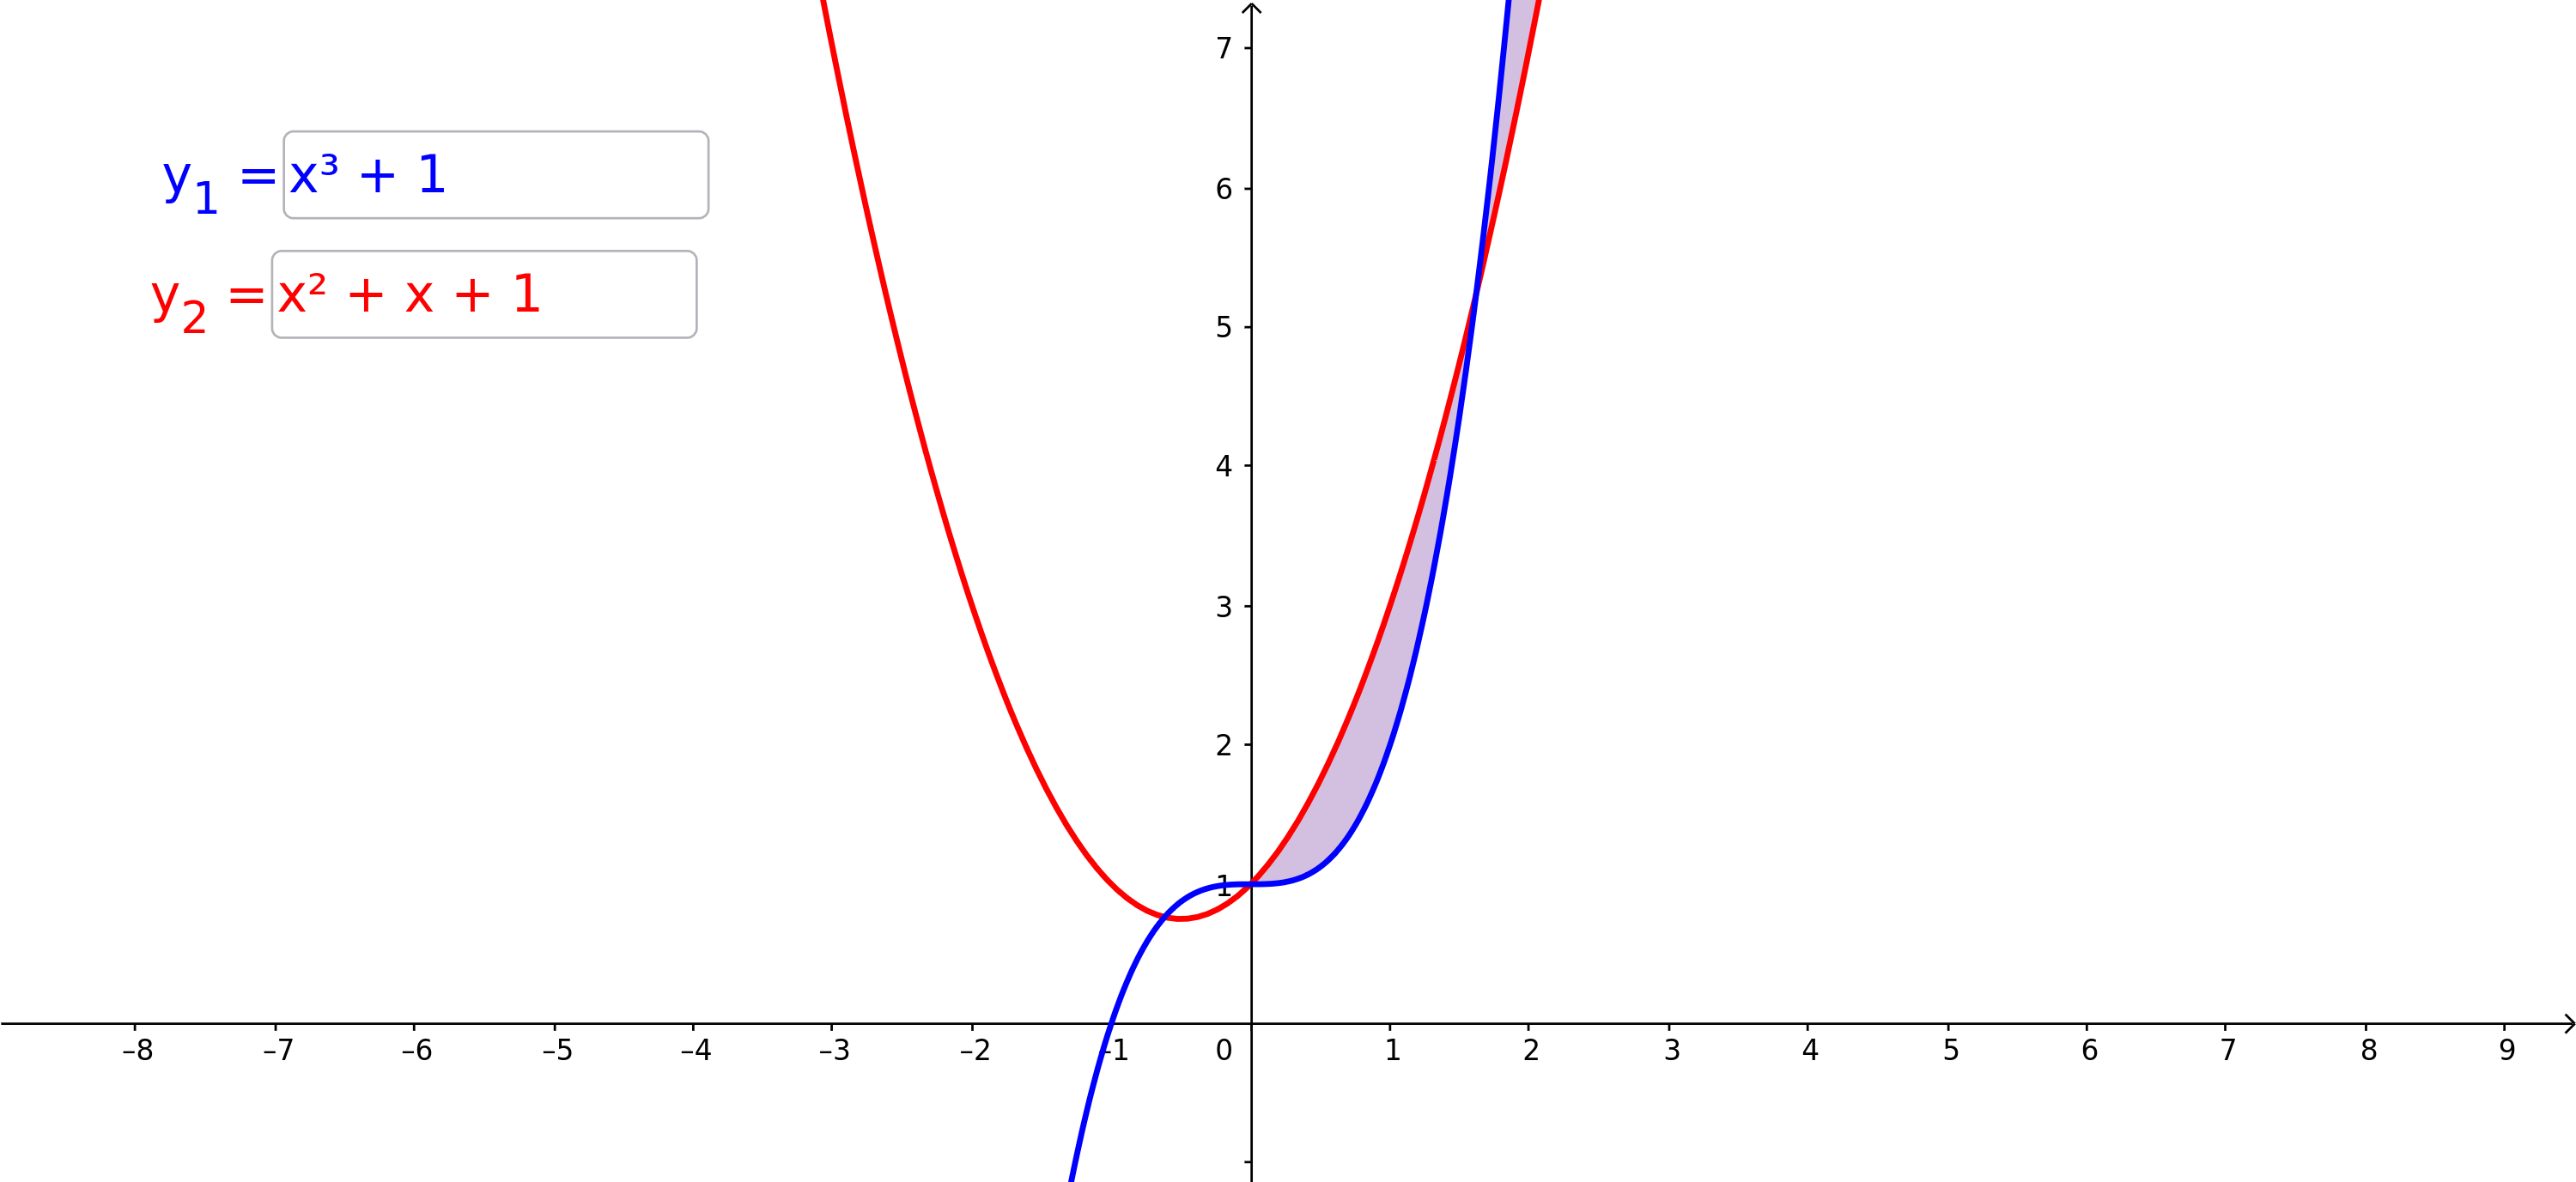
\includegraphics[width=10cm]{5D-4.11-sabawoon.enayat.INF.png}
\end{figure}

\begin{thebibliography}{999}
%\bibitem{a} Referentie
\end{thebibliography}
\end{document} 

